\documentclass{article}
\usepackage[utf8]{inputenc}
\usepackage{amsmath}
\usepackage{siunitx}
\usepackage{array}
\usepackage{multirow}
\usepackage[a4paper, total={6.5in, 9in}]{geometry}
\usepackage{graphicx}
\parindent=0pt

\DeclareSIUnit{\fahrenheit}{^\circ F}

\title{PHYS 157 Notes}
\author{Raymond Wang}
\date{October 2022}

\begin{document}

\maketitle

\tableofcontents

\section{Temperature}

\subsection{Temperature and Thermal Equilibrium}

\begin{itemize}
    \item Key terms: temperature, thermometer, thermal equilibrium, insulator, conductor.
\end{itemize}

\begin{itemize}
    \item The Zeroth Law of Thermodynamics: If $C$ is initially in thermal equilibrium with both $A$ and $B$, then $A$ and $B$ are also in thermal equilibrium with each other.
    \item Condition for Thermal Equilibrium: Two systems are in thermal equilibrium if and only if they have the same temperature.
\end{itemize}

\subsection{Temperature Scales}

\subsubsection{Celsius and Fahrenheit Scales}

\begin{itemize}
    \item Celsius temperature scale: water's freezing point is \SI{0}{\celsius} and water's boiling point is \SI{100}{\celsius}.
    \item Fahrenheit temperature scale: water's freezing point is \SI{32}{\fahrenheit} and water's boiling point is \SI{212}{\fahrenheit}.
\end{itemize}
\begin{align*}
    T_F &= \frac{9}{5}T_C + 32^\circ \\
    T_C &= \frac{5}{9}(T_F-32^\circ)
\end{align*}

\subsubsection{Kelvin Scale}

\begin{itemize}
    \item Has the same increments as the Celsius temperature scale, but \SI{0}{\kelvin} is defined at absolute zero. 
\end{itemize}
\[T_K=T_C+273.15\]
\begin{itemize}
    \item Can be defined using a gas thermometer and one reference temperature. 
\end{itemize}
\[\frac{T_2}{T_1}=\frac{p_2}{p_1}\]

\section{Thermal Expansion, Stress, and Strain}

\subsection{$\Delta L$ due to $\Delta T$}
\[\Delta L = \alpha L_0 \Delta T\]
\[L=L_0(1+\alpha\Delta T)\]
% $L$: length. $\alpha$: coefficient of linear expansion. $\Delta T$: change in temperature.

\subsection{$\Delta V$ due to $\Delta T$}
\[\Delta V = \beta V_0 \Delta T\]
\[V = V_0(1 + \beta \Delta T)\]
\[\beta = 3\alpha\]
% $V$: length. $\beta$: coefficient of volume expansion. $\Delta T$: change in temperature.

\subsection{Young's Modulus}
\[\frac{\Delta F}{A}=Y\frac{\Delta L}{L_0} \implies Y = \frac{\Delta F/A}{\Delta L/L_0}\]
\[\Delta L = \frac{L_0\Delta F}{YA}\]

\subsection{$\Delta L$ due to $\Delta T$ and $\Delta F$}
\[\Delta L = \Delta L_T + \Delta L_F = \alpha L_0\Delta T + \frac{L_0\Delta F}{YA}\]

\section{Heat and Temperature/Phase Change}
% Starting from page 552 in textbook

\subsection{Heat of Temperature Change}
\[Q=mc\Delta T\]

\subsection{Heat of Phase Change}
\[Q=\pm mL\]

\section{Heat Flow: Conduction and Convection}

\subsection{Heat Conduction}
\[H=\frac{dQ}{dt}=kA\frac{T_H-T_C}{L}\]

\subsection{Thermal Resistance}
\[R=\frac{L}{k}\]
\[H=\frac{A(T_H-T_C)}{R}\]
\begin{center}
    In layers (series): $R_{total}=R_1+R_2+\dots+R_n$ \\
\end{center}

\section{Radiation}

\subsection{Radiation}

\[H=Ae\sigma T^4\]
\[\sigma=\SI[per-mode=symbol]{5.67e-8}{\watt\per\meter\squared\per\kelvin\tothe{4}}\]

\subsection{Net Radiation}
\[H_{net}=Ae\sigma(T^4-T_s^4)\]

\subsection{Intensity at Distance $R$}
\[I=\frac{H}{A}=\frac{H}{4\pi R^2}\]
\[\frac{I_2}{I_1}=\left(\frac{R_1}{R_2}\right)^2\]

\subsection{Wien Displacement Law}
\[\lambda_{max}=\frac{b}{T}\]
\[b=\SI{2.90e-3}{\meter\kelvin}\]

\section{Thermodynamic Processes, Work, Heat, and Internal Energy}

\subsection{Ideal Gas Law}
\[pV=nRT\]

\subsection{Work Done by Gas}
\[W=F\Delta x_{\parallel}=\int_{x_1}^{x_2}F(x)dx\]
\[W=p\Delta V = \int_{V_1}^{V_2}p(V)dV\]

\subsection{First Law of Thermodynamics}
\[\Delta U=Q-W\]
\[Q=\Delta U+W\]
\begin{itemize}
    \item $\Delta U$: change in internal energy of the gas
    \item $Q$: heat added to gas
    \item $W$: work done by the gas
\end{itemize}
For cyclic processes, $\Delta U=0$, so $Q=W$.

\subsection{Internal Energy}
\[U=\frac{3}{2}nRT\text{ (monoatomic)}\] 
\[U=\frac{5}{2}nRT\text{ (diatomic)}\]
\[\Delta U = nC_V \Delta T\]
For all ideal gases, where $C_V=\frac{3}{2}R$ for monoatomic gases and $C_V=\frac{5}{2}R$ for diatomic gases.

\subsection{Thermodynamic Processes}
\subsubsection{Isochoric}
Constant volume process.
\[W=0\]
\[Q=\Delta U=nC_V\Delta T\]
\[Q=\left(\frac{C_V}{R}\right)V\Delta p\]

\subsubsection{Isobaric}
Constant pressure process. Can be indicated by "moveable piston."
\[W=p\Delta V\]
\[W=nR\Delta T\]
\[Q=\Delta U+W=nC_V\Delta T+nR\Delta T=nC_p\Delta T\]
\[Q=\left(\frac{C_p}{R}\right)p\Delta V\]
Where $C_p=C_V+R$.

\subsubsection{Isothermal}
Constant temperature process. Slow process where temperature is allowed to equilibrate with surroundings.
\[\Delta U=0\]
\[Q=W=nRT\ln\left(\frac{V_2}{V_1}\right)\]
\[Q=W=p_1V_1\ln\left(\frac{V_2}{V_1}\right)=p_2V_2\ln\left(\frac{V_2}{V_1}\right)\]

\subsubsection{Adiabatic}
No heat transfer. Fast process where there is no time for significant heat flow.
\[Q=0\]
\[\gamma=\frac{C_p}{C_V}\]
\[TV^{\gamma-1}=\text{ constant}\]
\[pV^{\gamma}=\text{ constant}\]
\begin{align*}
    W&=-\Delta U=nC_V(T_1-T_2) \\
    &= \frac{C_V}{R}(p_1V_1-p_2V_2) \\
    &= \frac{1}{\gamma-1} (p_1V_1-p_2V_2)
\end{align*}

\section{Cyclic Thermodynamic Processes, Heat Engines, and Refrigerators}

\subsection{Cyclic Processes}
\[\Delta U=0\]
\[Q=W\]
Sign convention: 
\begin{itemize}
    \item $Q$ is positive when it enters the engine/refrigerator and negative when it exits.
    \item $W$ is positive when there is work output and negative when there is work input.
\end{itemize} 

\subsection{Heat Engines}
\begin{itemize}
    \item $Q_H>0$: heat absorbed during one cycle 
    \item $Q_C<0$: heat rejected during one cycle 
    \item $W>0$: work output during one cycle 
\end{itemize}
\[Q=Q_H+Q_C=|Q_H|-|Q_C|\]
\[e=\frac{W}{Q_H}=1+\frac{Q_C}{Q_H}=1-\left|\frac{Q_C}{Q_H}\right|\]
\begin{center}
    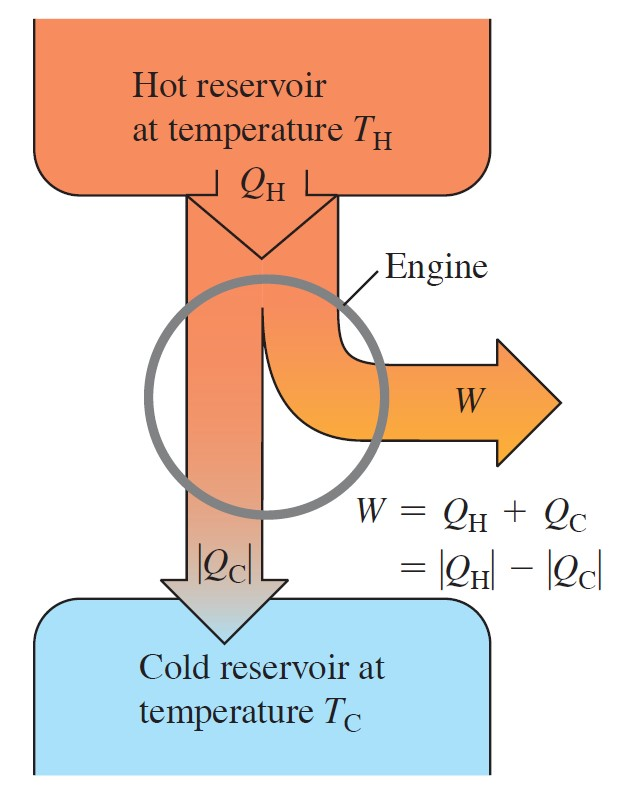
\includegraphics[scale=0.2]{images/heat_engine_energy_flow.jpg}
\end{center}

\subsubsection{Otto Cycle}
\[e=1-\frac{1}{r^{\lambda-1}}\approx 35\%\]
\begin{center}
    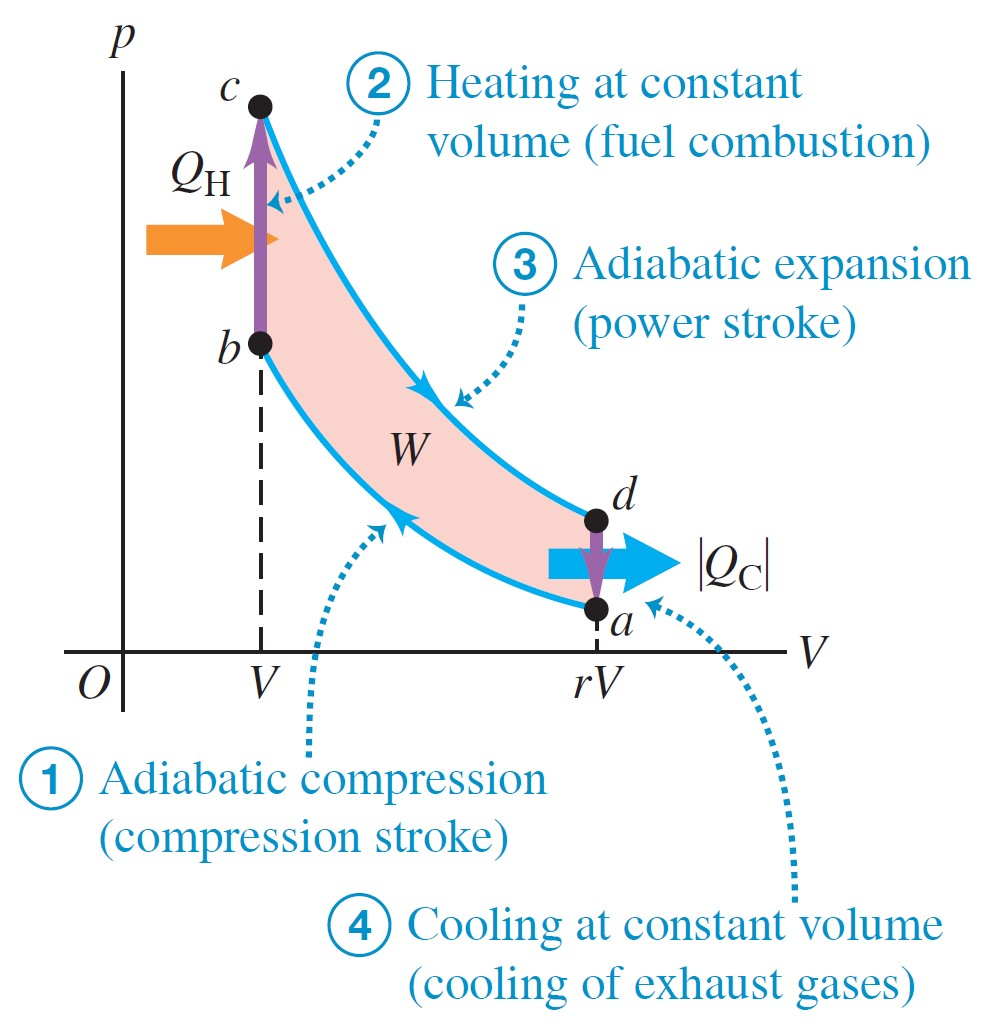
\includegraphics[scale=0.23]{images/otto_cycle.jpg}
\end{center}

\subsubsection{Diesel Cycle}
\begin{center}
    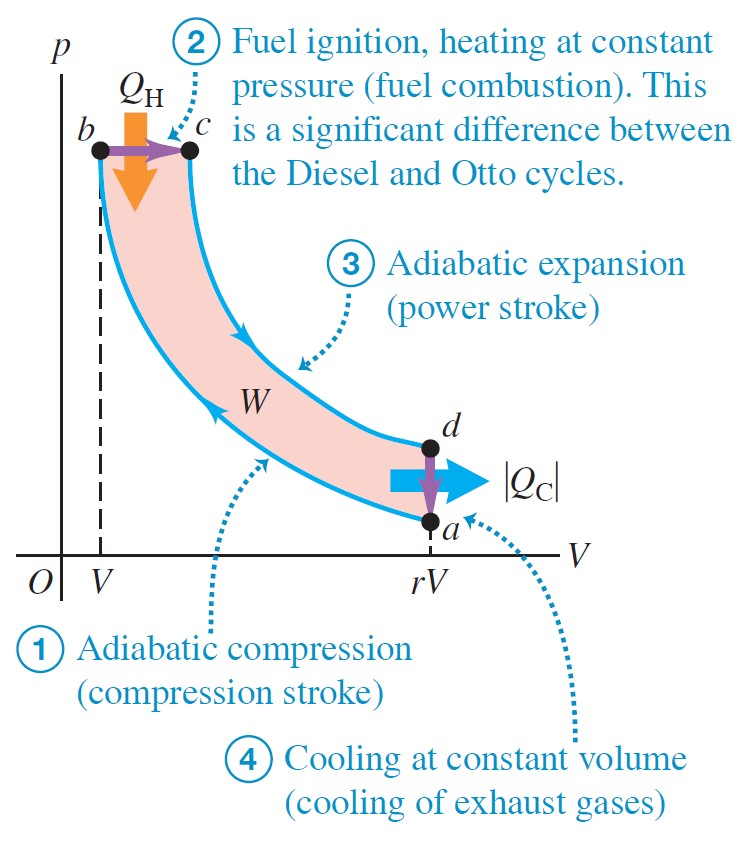
\includegraphics[scale=0.3]{images/diesel_cycle.jpg}
\end{center}

\subsection{Refrigerators}
\begin{itemize}
    \item $Q_H<0$: heat discarded to the hot system (outside air)
    \item $Q_C>0$: heat removed from cold system (refrigerator)
    \item $W<0$: work input of refrigerator 
\end{itemize}
\[Q=Q_H+Q_C=|Q_C|-|Q_H|\]
\[K=\frac{Q_C}{|W|}=\frac{|Q_C|}{|Q_H|-|Q_C|}\]
\begin{center}
    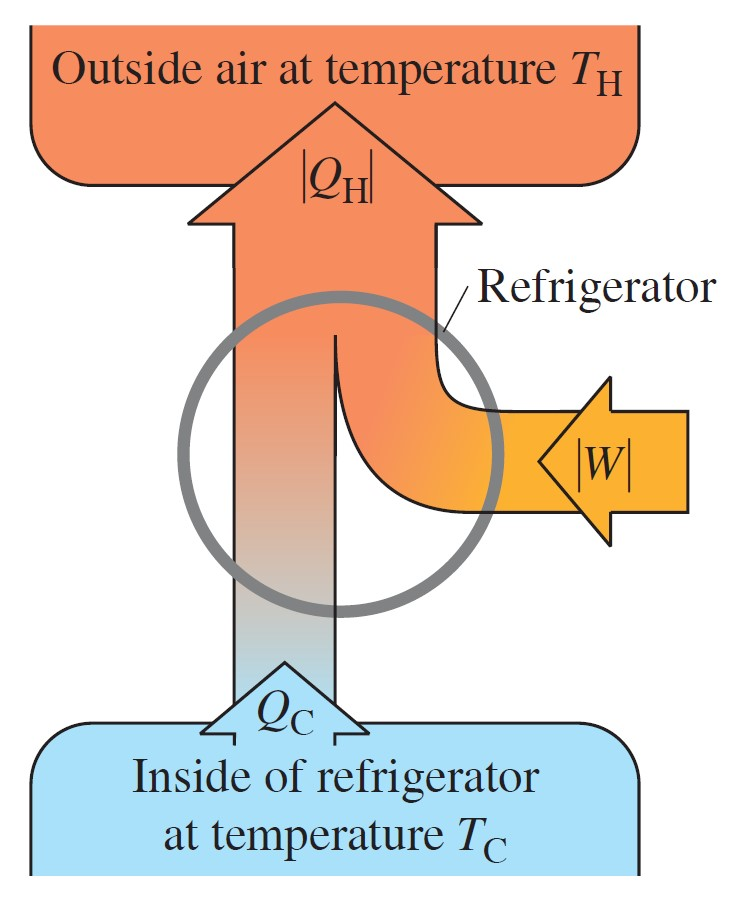
\includegraphics[scale=0.25]{images/refrigerator_energy_flow.jpg}
\end{center}

\section{Entropy}
\begin{itemize}
    \item A state variable that measures the disorder of a system. 
\end{itemize}

\subsection{Microscopic Definition of Entropy}
\[S=k\ln w\]
\begin{itemize}
    \item k: Boltzmann constant
    \item w: number of microstates of a given macrostate
\end{itemize}

\subsection{Macroscopic Definition of Entropy}
\[dS=\frac{dQ}{T}\]
\[\Delta S=\int_{1}^2 \frac{dQ}{T}\]
\[\Delta S=\frac{Q}{T} \text{ (reversible isothermal process)}\]

\subsection{Second Law of Thermodynamics}
The total entropy of a closed system never decreases.

\subsection{T-S Diagrams}
\begin{itemize}
    \item $Q_H$: area under curve
    \item $W$: area enclosed
\end{itemize}
\begin{center}
    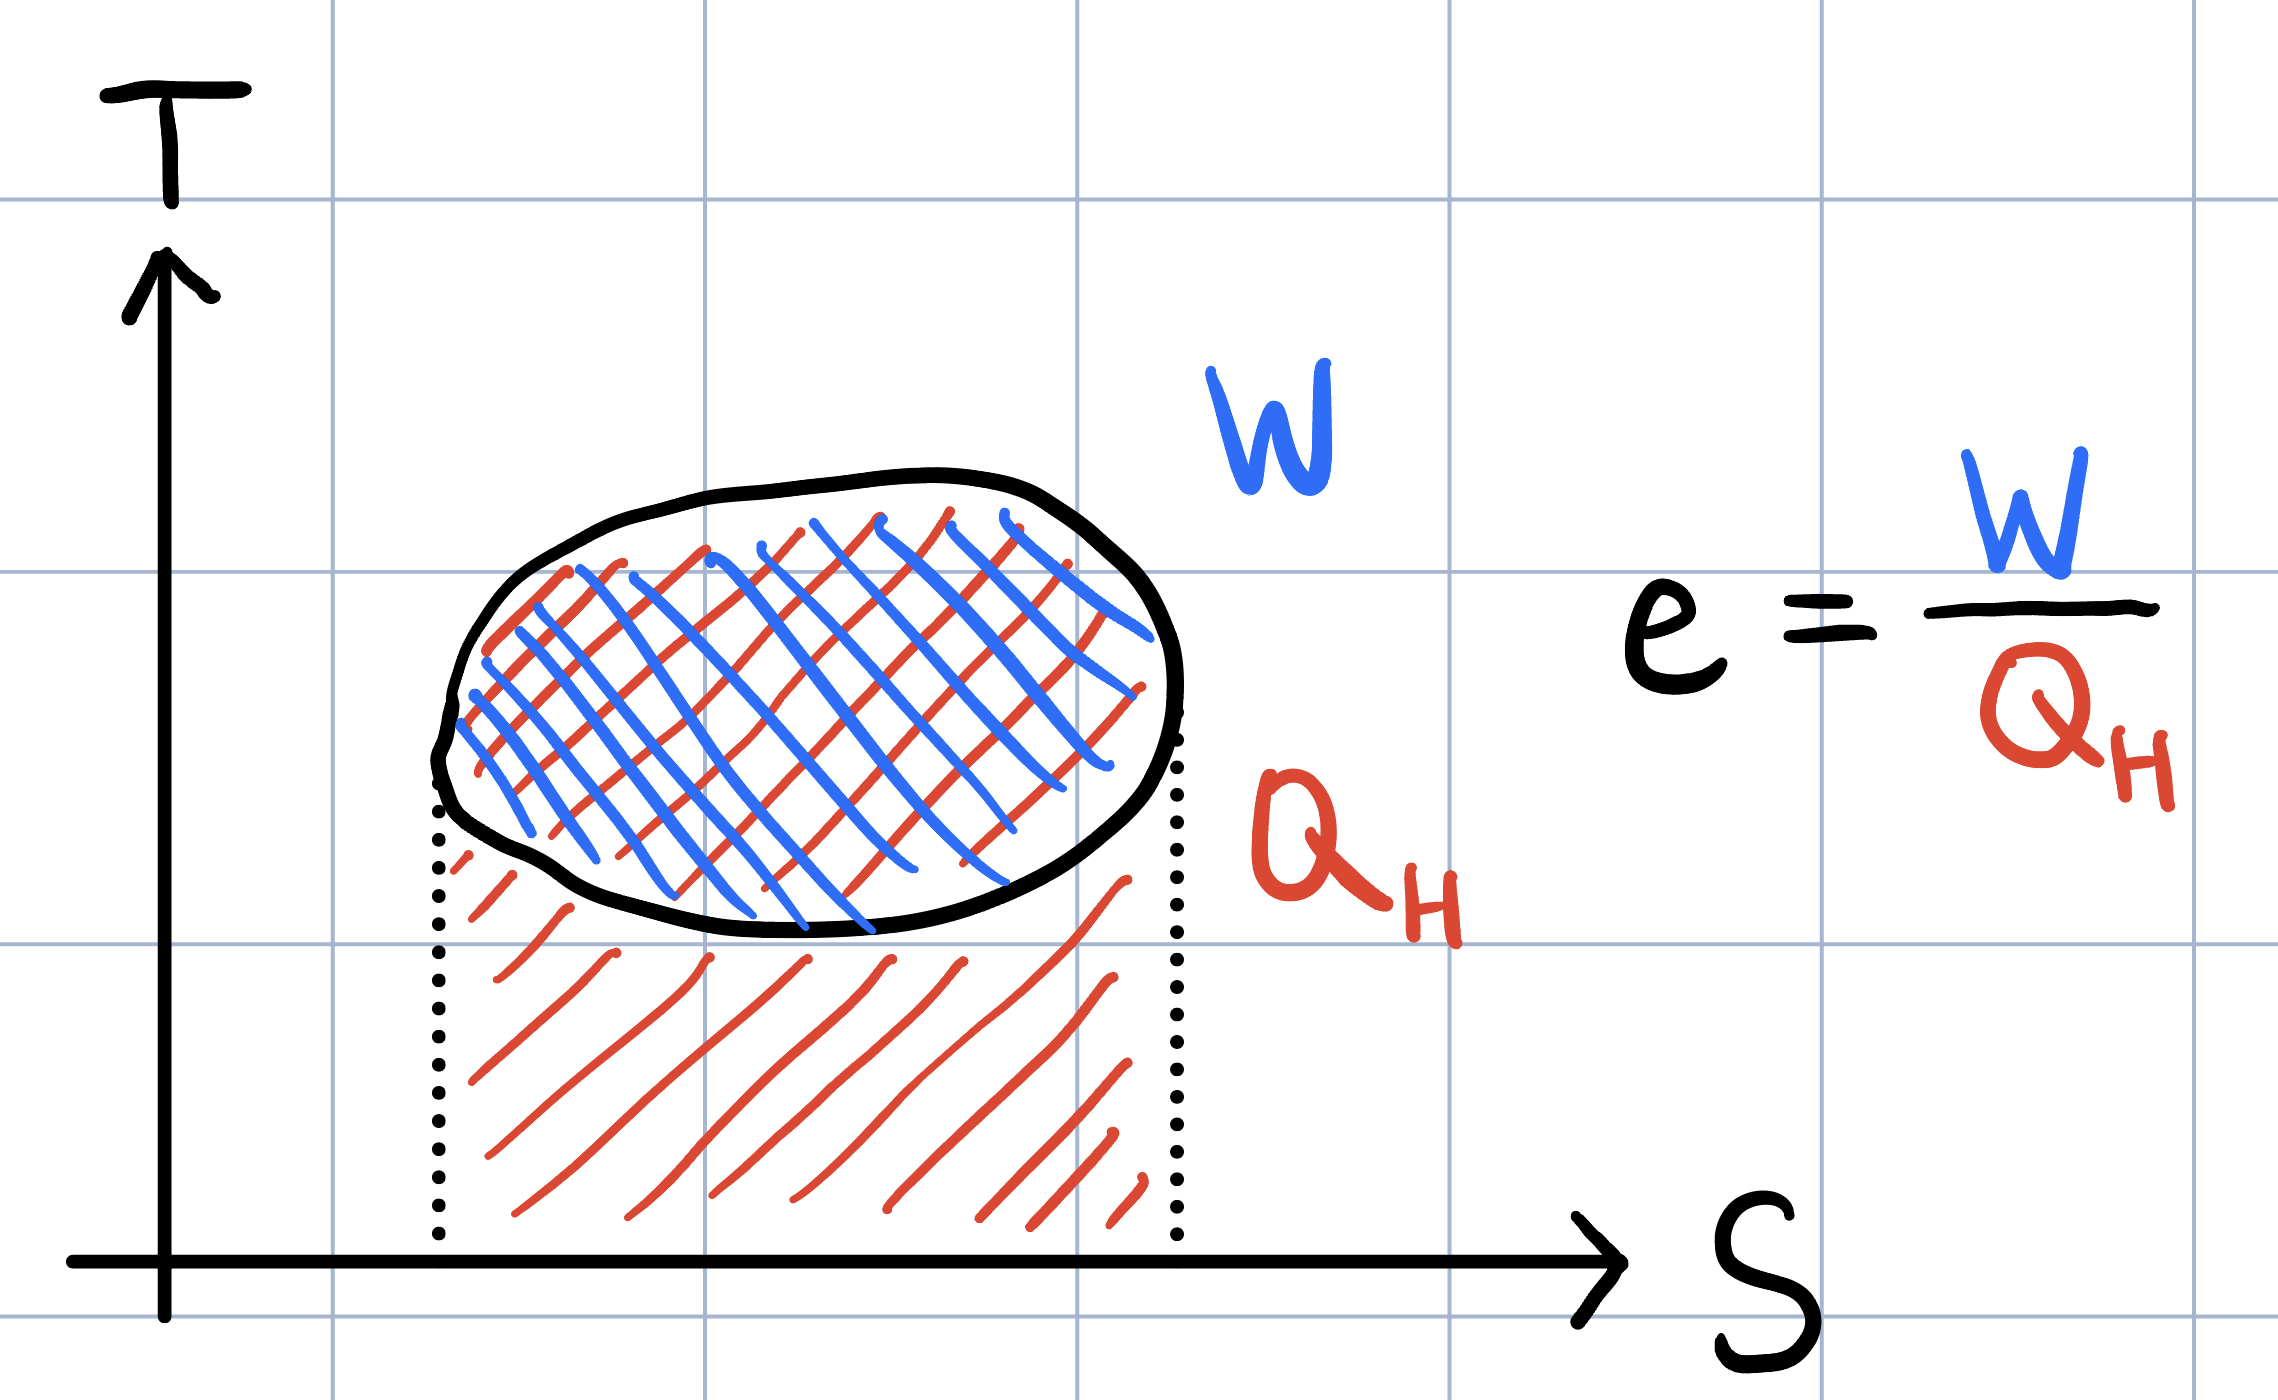
\includegraphics[scale=0.1]{images/T-S_diagram.jpg}
\end{center}

\subsection{Carnot Cycle}
\begin{itemize}
    \item Isothermal and adiabatic processes.
    \item Maximum efficiency of engine operating between temperatures of $T_H$ and $T_C$.
\end{itemize}
\begin{center}
    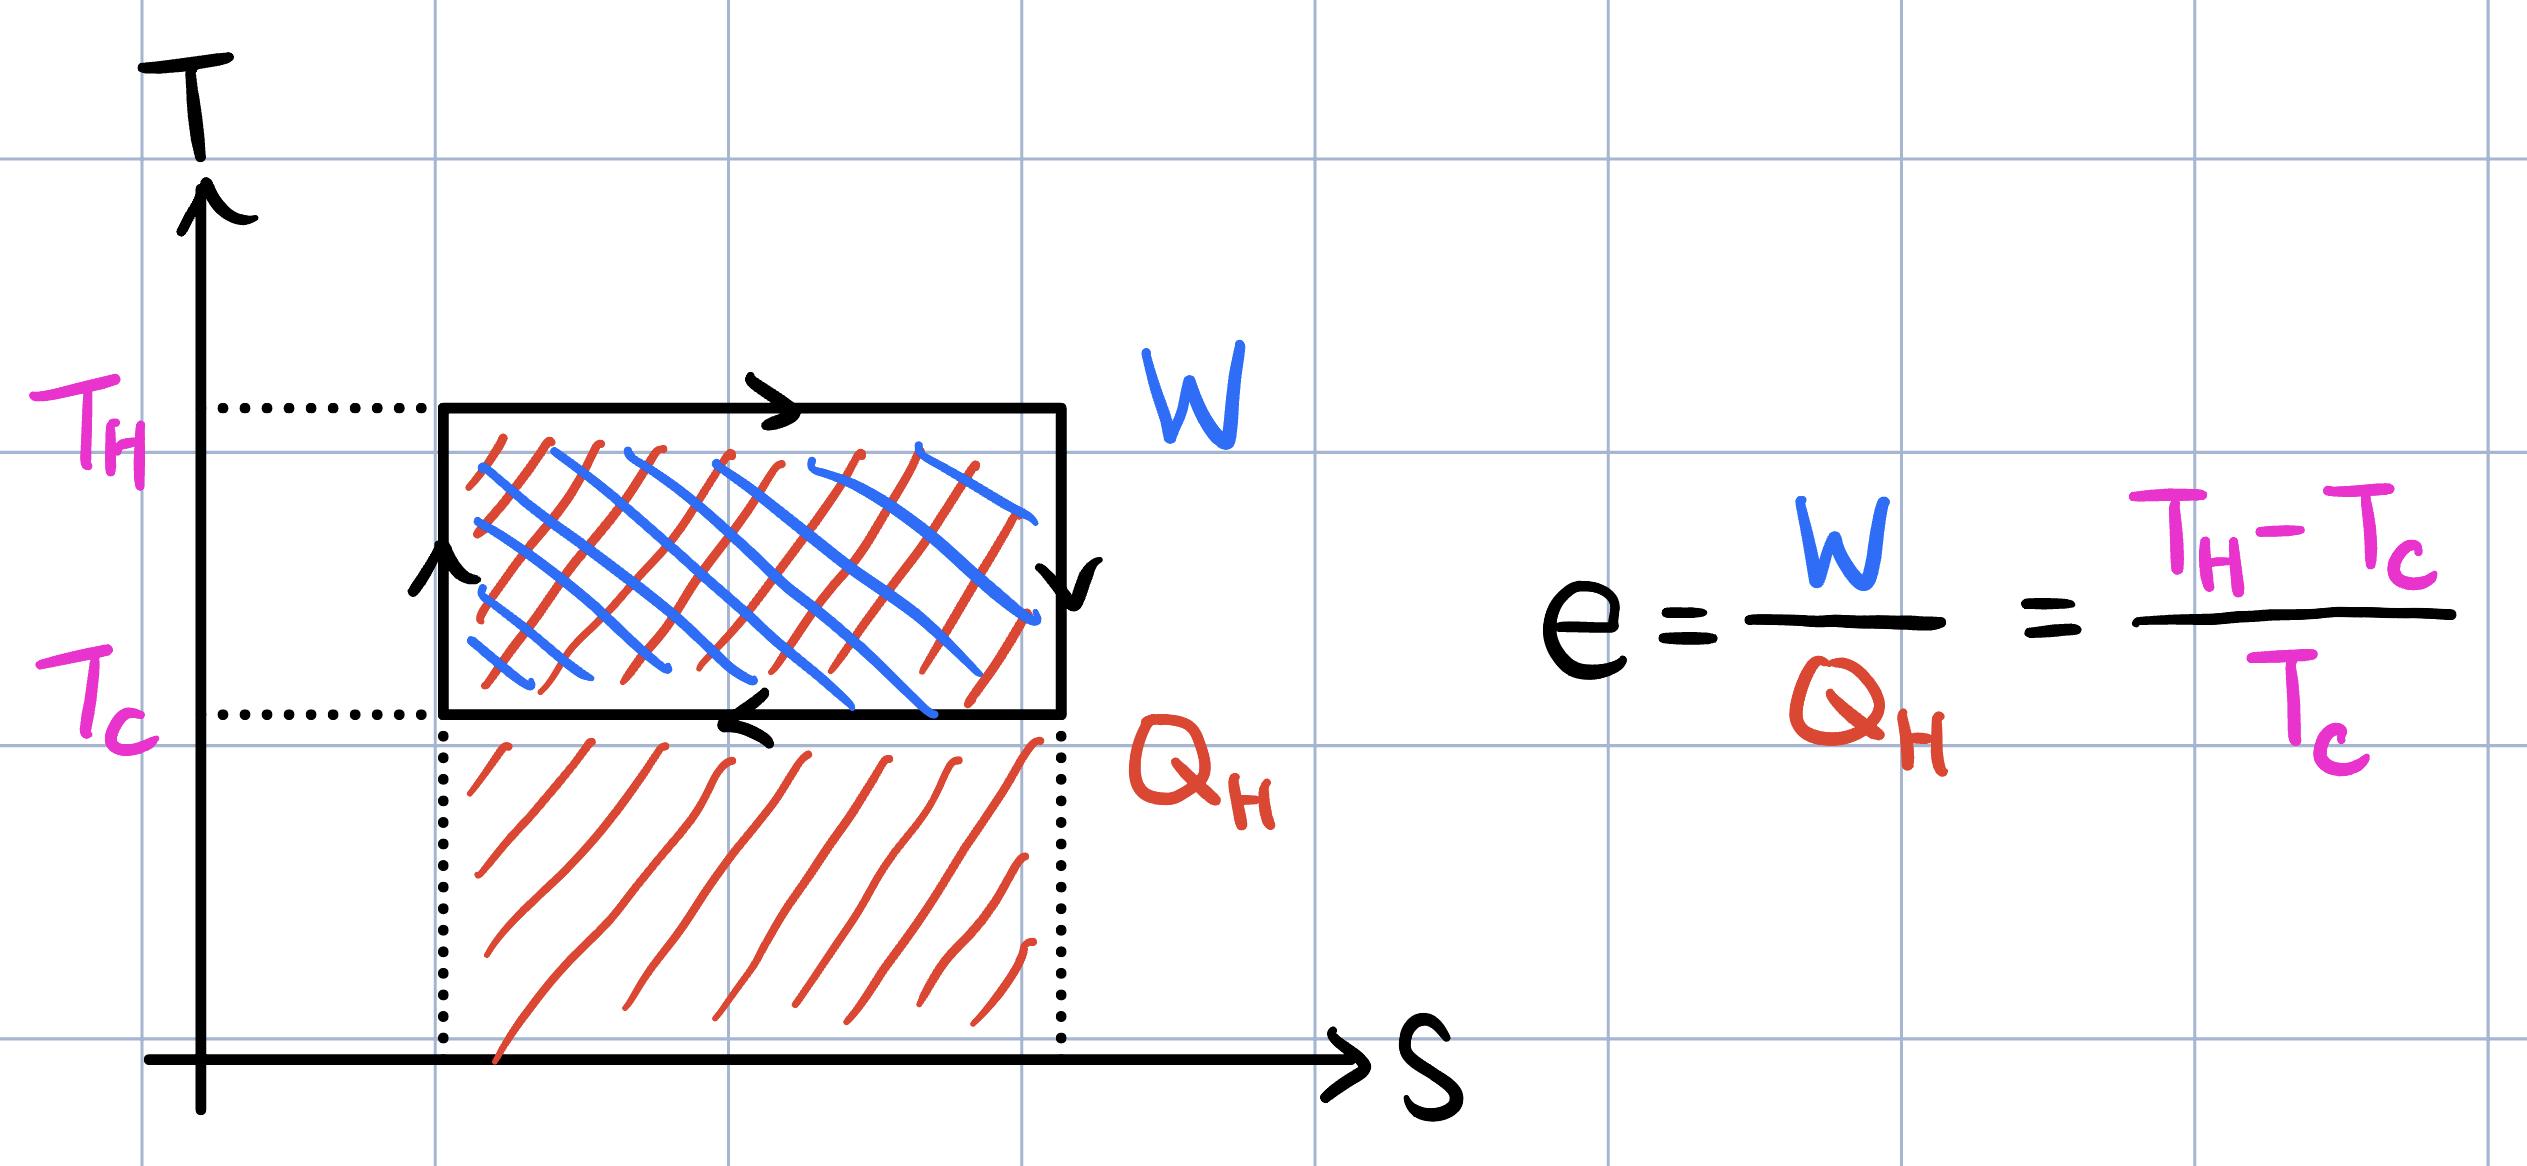
\includegraphics[scale=0.1]{images/carnot_cycle.jpg}
\end{center}

\section{Periodic Motion}

\subsection{Describing Oscillations}
\begin{itemize}
    \item $A$: amplitude = $|x|_{max}$.
    \item $T$: period = time to complete one cycle.
    \item $f$: frequency = number of cycles per unit time.
    \item $\omega$: angular frequency.
\end{itemize}
\[\omega=2\pi f=\frac{2\pi}{T}\]

\subsection{Simple Harmonic Motion}
\[F_x=-kx \text{ (Restoring Force)}\]
\[a_x=\frac{d^2x}{dt^2}=-\frac{k}{m}x\]
\[\omega=\sqrt{\frac{k}{m}}\]

\subsection{Displacement, Velocity, and Acceleration}
\[x=A\cos(\omega t+\phi)\]
\[v=-\omega A\sin(\omega t+\phi)\]
\[a=-\omega^2 A\cos(\omega t+\phi)\]
Plug in $x_0$ to find $\phi$.

\subsection{Energy in Simple Harmonic Motion}
\[E=\frac{1}{2}mv^2+\frac{1}{2}kx^2=\frac{1}{2}kA^2=\text{ constant}\]

\subsection{Damped Oscillations}
\[F_x=-kx-bv_x \text{ (restoring and damping/drag force)}\]
\[t_0=\frac{2m}{b}, t_0=-\frac{T}{\ln(r)} \text{ (where $r$ = reduction fraction per period)}\]
\[x=Ae^{-t/t_0}\cos(\omega' t+\phi)\]
\[\omega'=\sqrt{\frac{k}{m}-\frac{b^2}{4m^2}}\]
\begin{itemize}
    \item Critical damping: $b=2\sqrt{km}$
    \item Overdamping: $b>2\sqrt{km}$ (returns to equilibrium slower than critical damping)
\end{itemize}

\subsection{Effective Spring Constant}
\[k=-\frac{dF_{net}}{dx}(x_{eq})\]

\section{Waves}
\begin{itemize}
    \item Transverse wave: displacement is perpendicular to direction of travel
    \item Longitudinal wave: displacement is in the same direction as direction of travel 
    \item $v$: wave speed. Speed of disturbance propagation
\end{itemize}

\subsection{Periodic Waves}
\[v=\lambda f\]

\end{document}
